\section{Performance comparison of Hadoop vs. Linux} \label{T2}

\paragraph{}To perform this comparison, we run the WordCount script 10 time for both Hadoop and Linux to get an approximate average run-time for each. These tests were made on the AWS Instance. However, the same tests have been done locally and results were confirmed the ones showed bellow. Here is a graph comparing those two metrics.
\begin{center}
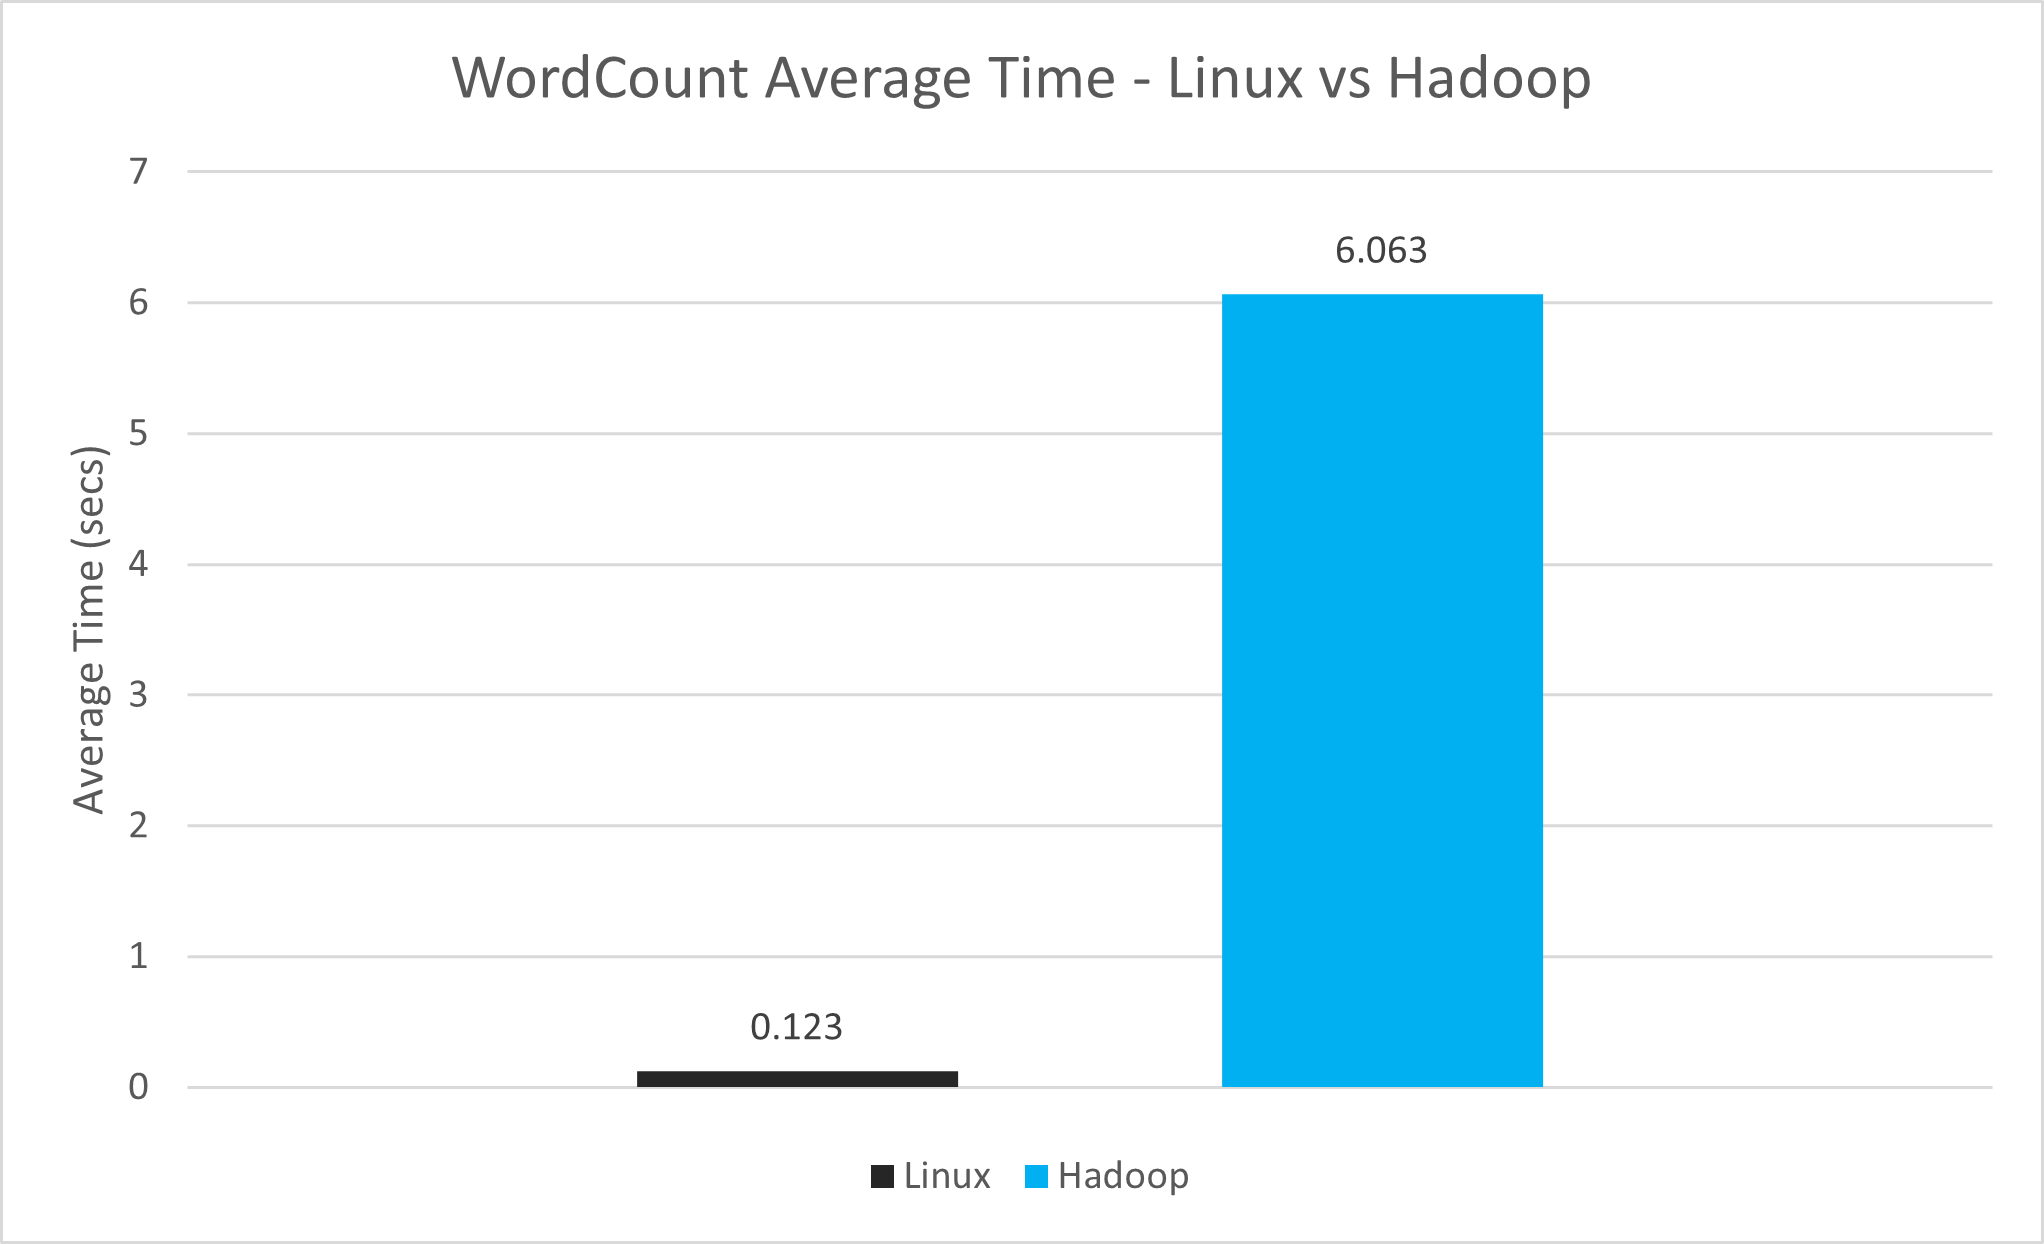
\includegraphics[width=14cm]{Resources/linux_vs_hadoop.png}\\
\emph{Figure 2.1 - Linux vs Hadoop average time}
\end{center}
\paragraph{}From the above graph, we can conclude that Linux is about 50 time faster than Hadoop. This can be explained by the fact that Hadoop works on the the disk, unlike Linux script which runs in memory. Here, the dataset is not big enough for Hadoop to outperform Linux, and the initialization phase of Hadoop alone is enough to make it way slower than the Linux script.